%% 30min talk

\documentclass[english]{beamer}
\usetheme{Warsaw}
\setbeamertemplate{navigation symbols}{} % remove the navigation symbols
\setbeamertemplate{headline}{} % remove headline
\setbeamertemplate{footline}[frame number]

\usepackage{babel}
\usepackage[utf8]{inputenc}
\usepackage{textcomp}
\usepackage{wasysym}
\usepackage{diagmac2}
\usepackage{cancel}

\title{Beyond-the-standard-model contributions to rare B decays analyzed with variational-Bayes enhanced adaptive importance sampling}
\author{Stephan Jahn}
\date{March 16, 2015}

% ----------------------------------------------------------------------

\newcommand{\slide}[2][t]{\begin{frame}[#1] \frametitle{\insertsection} #2 \end{frame}}
\newcommand{\KLPp}[0]{KL( P\|{}p)}
\newcommand{\KLqp}[0]{KL( q\|{}p)}
\newcommand{\varmuN}{var(\mu^{N})}
\newcommand{\wilsoncten }{\mathcal{C} ^{      } _{10}}
\newcommand{\wilsonctenp}{\mathcal{C} ^{\prime} _{10}}
\newcommand{\errorasymm}[3]{#1 \substack{\hspace{.05em} \scriptscriptstyle + \hspace{.05em} #2 \\ \scriptscriptstyle -#3} } % asymmetric uncertainties
\newcommand{\gauss}{\mathcal{N}}
\newcommand{\diffd}[1]{\mbox{d} #1 \,} % differential d
\newcommand{\dx}{\diffd{x}}
\newcommand{\samples}{\boldsymbol{X}}
\newcommand{\red}[1]{\textcolor{red}{#1}}

\setbeamercolor{block title}{bg=blue, fg=white}

\begin{document}

% ----------------------- title page, unnumbered -----------------------

{
\setbeamertemplate{footline}{}
\frame[nopagenumbering,noframenumbering]{\titlepage}
}

% -------------------------- overview section --------------------------

\section{Overview}

\slide[t]{

    Bayes' formula:
    \newline \newline
    $$ P(\boldsymbol{\theta} | \mathcal{D}, \mathrm{M} ) = \frac{P(\mathcal{D}|\boldsymbol{\theta}, \mathrm{M})P(\boldsymbol{\theta} | \mathrm{M})}{P(\mathcal{D} | \mathrm{M} )}
       = \frac{P(\mathcal{D}|\boldsymbol{\theta}, \mathrm{M})P(\boldsymbol{\theta} | \mathrm{M})}{\int P(\mathcal{D}|\boldsymbol{\theta}, \mathrm{M})P(\boldsymbol{\theta} | \mathrm{M}) d\boldsymbol{\theta} }$$

    \only<2->{ \
        \newline \newline \
        our application: \
        \
        \newline \newline \

        \only<3->{$$ \boldsymbol{\theta} = \lbrace \mathcal{C}_{7 , 9 , 10 , S , P , T , T5}^{(\prime)}  , ... \rbrace $$}
        \only<4->{$$ \mathcal{D} = \mathrm{detector~events} $$}
        \only<5->{$$ \mathrm{M} = \mathrm{EFT , SM , ...} $$}
    }

}


\slide[t]{

{\large\textbf{Goals}}

\begin{columns}[t] % The "c" option specifies centered vertical alignment while the "t" option is used for top vertical alignment

\column{.45\textwidth} % Left column and width

\only<2->{\begin{itemize}
              \item draw marginal plots of the posterior
              \
              \newline

              \hspace{-1.2cm} 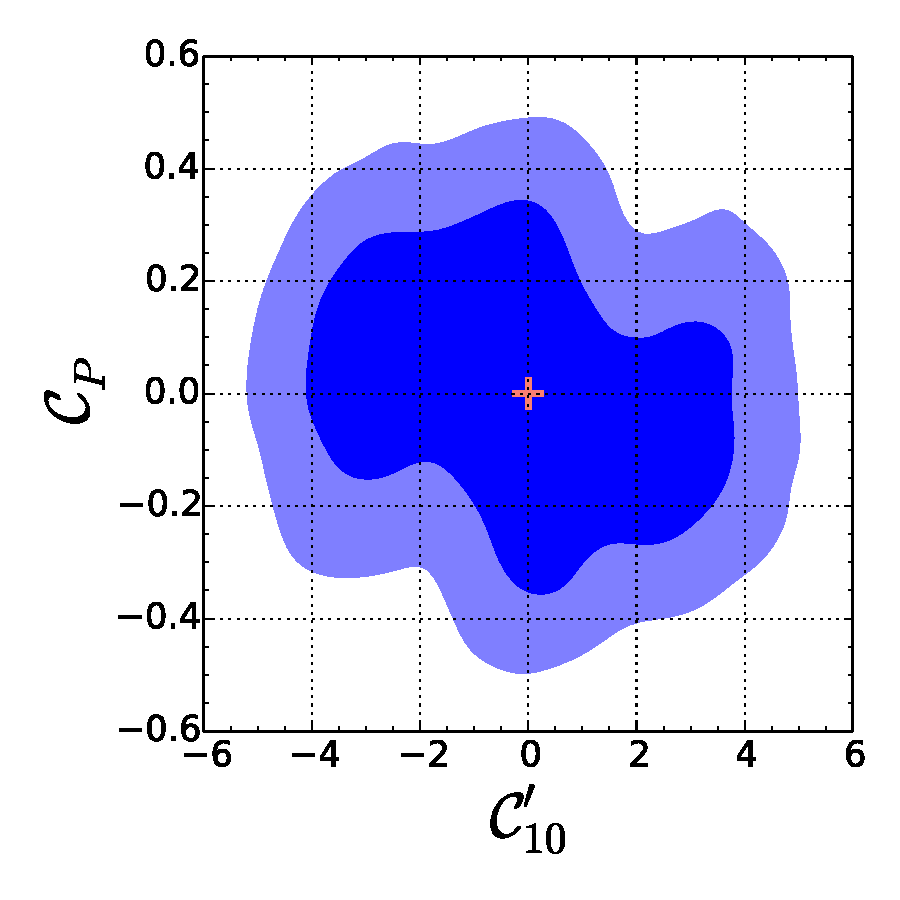
\includegraphics[width=1.01\textwidth]{figures/C10p_CP}

          \end{itemize}}

\column{.5\textwidth} % Right column and width

\only<3->{\begin{itemize}
          \item compare models \newline $\mathrm{NP} \leftrightarrow \mathrm{SM}$
          \end{itemize}

              $$ \frac{P(\mathrm{NP}|\mathcal{D})}{P(\mathrm{SM}|\mathcal{D})} =
                 \frac{P(\mathcal{D}|\mathrm{NP})}{P(\mathcal{D}|\mathrm{SM})} \cdot \frac{P(\mathrm{NP})}{P(\mathrm{SM})} $$

              $$ P(\mathrm{M} | \mathcal{D} ) = \frac{P(\mathcal{D} | \mathrm{M})P(\mathrm{M})}{P(\mathcal{D})} $$

          \begin{itemize}
          \item[]
              \begin{itemize}
                  \item[] \only<4->{\hspace{-0.1\textwidth} $\frac{P(\mathrm{NP}|\mathcal{D})}{P(\mathrm{SM}|\mathcal{D})} > 1$ new physics \smiley{} \newline}
                  \item[] \only<5->{\hspace{-0.1\textwidth} $\frac{P(\mathrm{NP}|\mathcal{D})}{P(\mathrm{SM}|\mathcal{D})} < 1$ confirm SM \frownie{}}
              \end{itemize}
          \end{itemize}}

\end{columns}

}





\slide[t]{

{\large\textbf{Difficulties}}

\begin{columns}[t] % The "c" option specifies centered vertical alignment while the "t" option is used for top vertical alignment

\column{.45\textwidth} % Left column and width

\vspace{0.65cm} % to center the text

\only<2->{\begin{itemize}}
\only<2->{\item curse of dimensionality}
\only<3->{\item multimodality}
\only<4->{\item degeneracies}
\only<2->{\end{itemize}}

\only<5->{\Huge \textcolor{red}{no standard algorithm so far}}

\column{.5\textwidth} % Right column and width

\vspace{-8mm}

\begin{center}
\only<3->{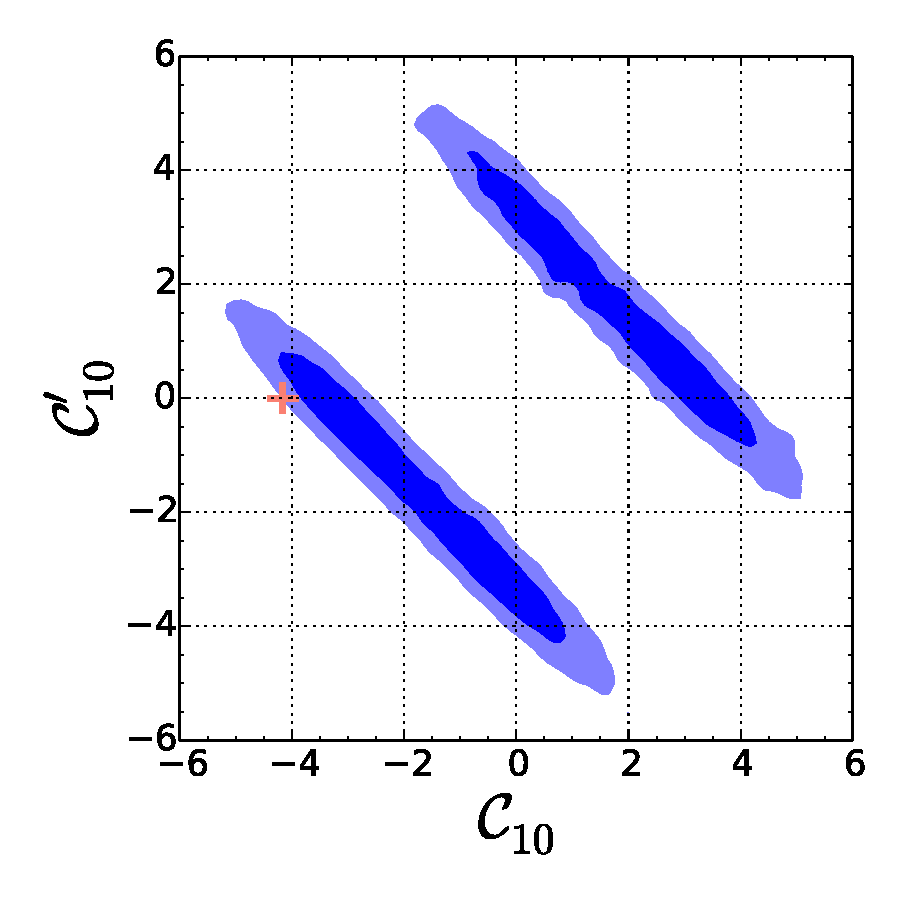
\includegraphics[height=0.4\textheight]{figures/C10_C10p}}

\only<4->{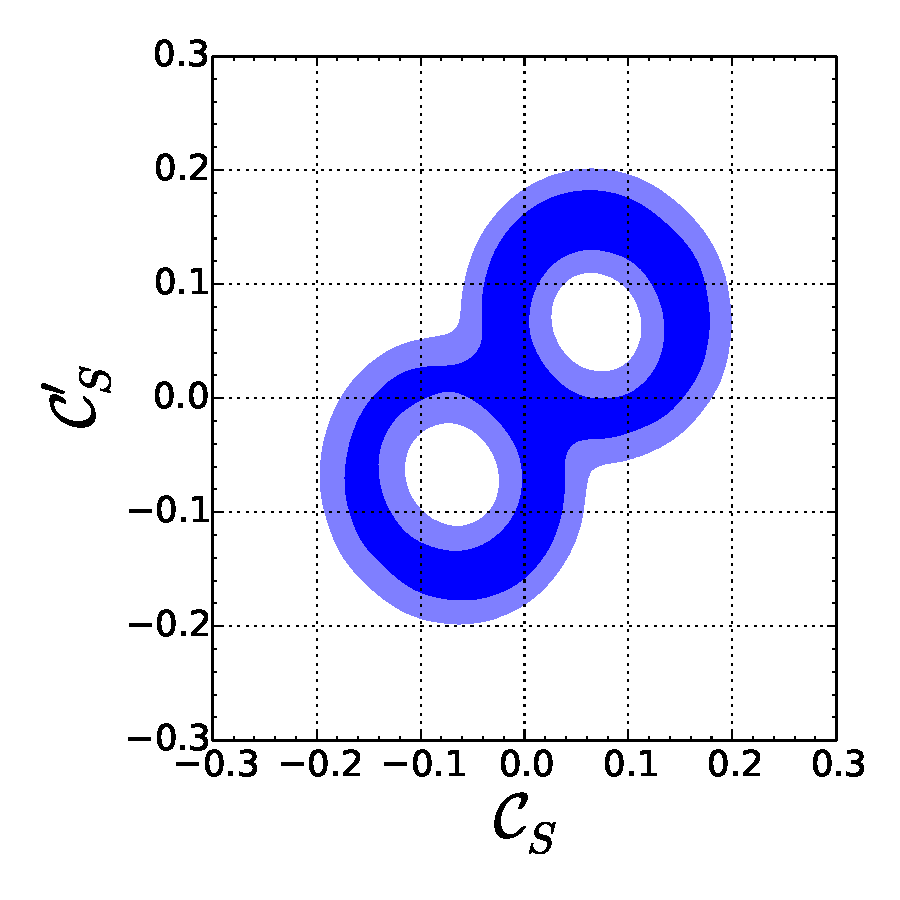
\includegraphics[height=0.43\textheight]{figures/example_for_degeneracy}}
\end{center}


\end{columns}

}

% ------------------------------ toc page ------------------------------

\begin{frame}
\frametitle{Contents}
\tableofcontents
\end{frame}

% ----------------------------- VB section -----------------------------

\section{Adaptive importance sampling with the variational-Bayes approach}

\begin{frame}
\frametitle{\insertsectionhead}
\tableofcontents[currentsection]
\end{frame}

\slide[c]{

    \frametitle{Adaptive importance sampling}

    $$ \int P(x) \dx = \int \frac{P(x)}{p(x)} p(x) \dx
    \approx \frac{1}{N} \sum^{N}_{n = 1} \frac{P(x_n)}{p(x_n)} \equiv \mu^{{N}} ~~ where ~~ x_n \sim p $$


    \uncover<2->{squared uncertainty (variance):

    $$ \varmuN = \frac{1}{N} \left[ \int \frac{P(x)}{p(x)} P(x) \dx - \left(\int P(x) \dx \right)^2 \right] $$}

    \uncover<3->{\Huge\begin{center}\red{minimize the uncertainty $\varmuN$ with respect to $p$}\end{center} }

}

\slide[c]{

    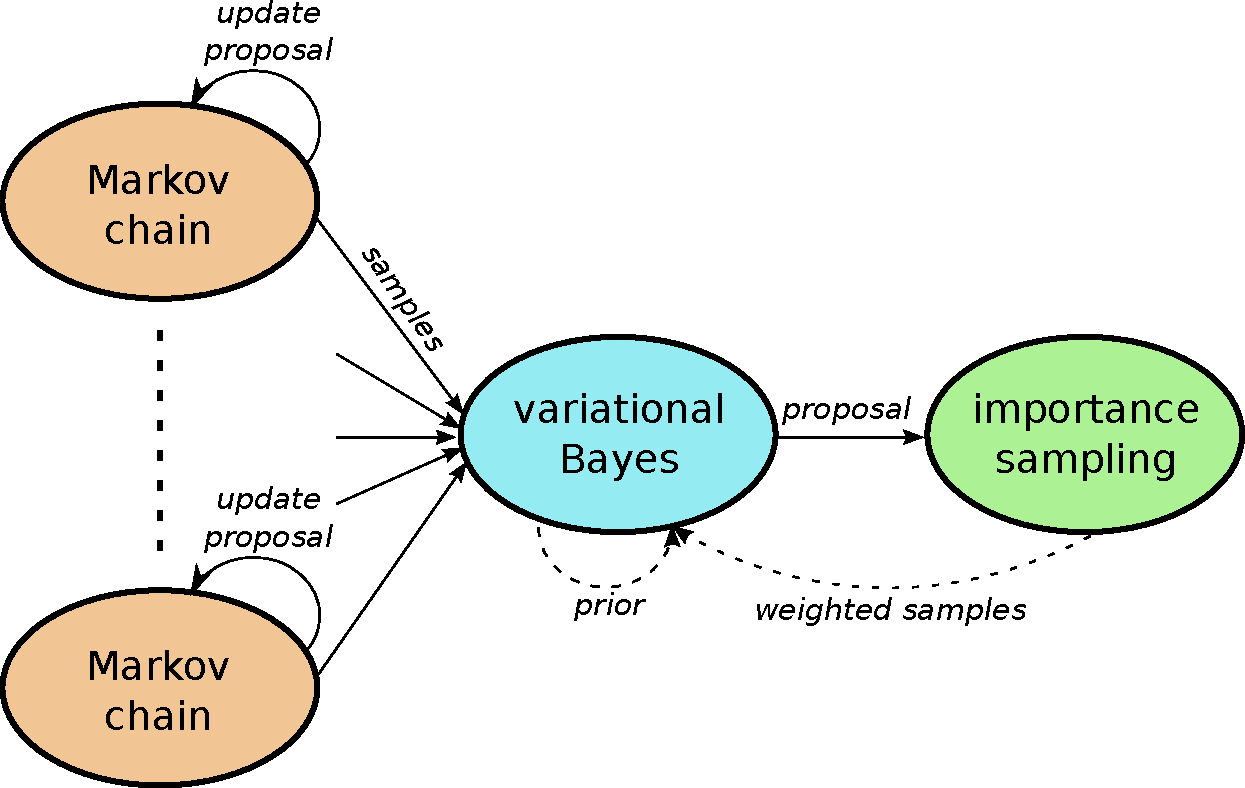
\includegraphics[width=\textwidth]{figures/algorithm}

}

\slide{

    \frametitle{{\fontfamily{qcr}\selectfont pypmc}}

    \vspace{3mm}

    %                                         trim= l b r t  ; crop the (not clickable) link on top and write it below
    \includegraphics[width=\textwidth,page=6, trim= 0 0 0 5cm, clip]{figures/presentation_22_april}



    \begin{center}
        \url{https://pypi.python.org/pypi/pypmc}
    \end{center}

}

% ------------------------- B-physics section --------------------------

\renewcommand{\slide}[2][t]{\begin{frame}[#1] \frametitle{\insertsubsectionhead} #2 \end{frame}}

\section{Scalar and tensor contributions to $ b \to s \mu^+ \mu^- $}

\begin{frame}
\frametitle{\insertsectionhead}
\tableofcontents[currentsection]
\end{frame}

\newcommand{\redsecond}[1]{\uncover<2->{\textcolor{red}{#1}}}
\slide{

    \frametitle{Effective theory}

    effective Lagrangian for $ b \to s \ell^+ \ell^- $ (\only<1>{$\mathrm{SM}$}\only<2>{\red{beyond}-$\mathrm{SM}$}): \
    \
    \newline \newline \

    $$ \mathcal{L}_{int} = \frac{4 G_F}{\sqrt{2}} \frac{\alpha_e}{4\pi} V_{tb}^{} V_{ts}^\ast \sum_i \mathcal{C}_i \mathcal{O}_i + ... + \text{h.c.} $$

    ~ \newline

    \begin{center}
      \begin{tabular}{cc}
          \small $ \mathcal{O}_{9} ^{\redsecond{(\prime)}} = \left[\bar{s} \gamma_\mu^{} P_{L\redsecond{(R)}} b\right]\!\left[\bar{\ell} \gamma^\mu \ell\right] $
                & \small $  \mathcal{O}_{10}^{\redsecond{(\prime)}} = \left[\bar{s} \gamma_\mu^{} P_{L\redsecond{(R)}} b\right]\!\left[\bar{\ell} \gamma^\mu \gamma_5 \ell\right] $ \\[1cm]
          \Large $ \begin{aligned}
                \redsecond{\mathcal{O}_S^{(\prime)}}    & \redsecond{= \left[\bar{s} P_{R\redsecond{(L)}} b\right]\!\left[\bar{\ell} \ell\right]} \\[5mm]
                \redsecond{\mathcal{O}_T}               & \redsecond{= \left[\bar{s} \sigma_{\mu\nu}^{} b\right]\!\left[\bar{\ell} \sigma^{\mu\nu} \ell\right] }
          \end{aligned} $ & \Large $ \begin{aligned}
                \redsecond{\mathcal{O}_P^{(\prime)}}    & \redsecond{= \left[\bar{s} P_{R(L)} b\right]\!\left[\bar{\ell} \gamma_5 \ell\right] } \\[5mm]
                \redsecond{\mathcal{O}_{T5}}            & \redsecond{= \left[\bar{s} \sigma_{\mu\nu}^{} b\right]\!\left[\bar{\ell} \sigma^{\mu\nu} \gamma_5 \ell\right] }
          \end{aligned} $
     \end{tabular}
    \end{center}

}

\newcommand{\sqrtqsq}{\sqrt{q^2}}
\slide{

    \frametitle{Sensitive observables}

    \begin{itemize}

        \item {\large\textbf{$\boldsymbol{B\rightarrow K\mu^+\mu^-}$ angular distribution} }

        \uncover<2->{$$
            \frac{1}{\Gamma} \frac{\mbox{d}\Gamma}{\mbox{d}\!\cos\theta}
            = \frac{3}{4} (1 - \red{F_H}) \sin^2\!\theta
            + \frac{1}{2} \red{F_H}
            + \red{A_{FB}} \cos\theta
        $$}

        \uncover<3->{$$ F_{H}^\mathrm{SM} = \mathcal{O}(m_\ell ^2/ q^2) ~~~~~ A_{FB}^\mathrm{SM} = 0 $$}

        \vspace{1.5cm}

        \item {\large\textbf{$\boldsymbol{B_s\rightarrow \mu^+\mu^-}$ branching fraction} }

        \vspace{-4mm}

        \uncover<4->{\begin{align*}
            \red{\mathcal{B}(B_s\rightarrow\mu^+\mu^-)} \propto | \mathcal{C}_{S} - \mathcal{C}_{S} ^\prime |^2 +
            |( \mathcal{C}_{P} - \mathcal{C}_{P} ^\prime ) + \frac{2 m_\ell}{M_{B_s}}( \wilsoncten - \wilsonctenp ) |^2
        \end{align*}}

    \end{itemize}

}

\slide{

    \frametitle{Methodology}

    we want:
    \newline
    $$ P(\boldsymbol{\theta} | \mathcal{D}, \mathrm{M} ) \overset{\mathrm{Bayes}}{\propto} P(\mathcal{D}|\boldsymbol{\theta}, \mathrm{M})P(\boldsymbol{\theta} | \mathrm{M}) $$

    \only<2->{

        \vspace{1.6mm}

        split theory and experiment - \emph{observables} $\boldsymbol{O}$:

        \only<-5|handout:0>{$$ P(\mathcal{D}|\boldsymbol{\theta}, \mathrm{M})
          = P(\mathcal{D} | \boldsymbol{O} (\boldsymbol{\theta} , \mathrm{M} )) $$}

        \only<6->{$$ P(\mathcal{D}|\boldsymbol{\theta}, \mathrm{M})
          = P(\mathcal{D} | \boldsymbol{O} (\boldsymbol{\theta} , \mathrm{M} ) , \underset{ \text{\textcolor{red}{\textbf{assumption} }} } {\cancel{\boldsymbol{\textcolor{red}{\theta , \mathrm{M}}}}} ) $$}

        \vspace{-6.5mm}

        \only<3->{

            \begin{center}
                \begin{columns}[t] % the "t" option specifies top vertical alignment

                    \column{.5\textwidth}
                        \begin{block}{\center theory}
                            \begin{center}
                                \only<-3|handout:0>{ ~ \vspace{8.4mm} ~ }
                                \only<4->{~~~\emph{calculate} observables \newline
                                $ \boldsymbol{O}(\boldsymbol{\theta} , \mathrm{M}) $}
                            \end{center}
                        \end{block}
                        \only<4->{\center 
\includegraphics[height=1.5cm]{figures/theorist}}

                    \column{.5\textwidth}
                        \begin{block}{\center experiment}
                            \begin{center}
                                \only<-4|handout:0>{ ~ \vspace{8.4mm} ~ }
                                \only<5->{~~~~~\emph{measure} observables \newline
                                    \only<-5|handout:0>{$P\left(\mathcal{D} | \boldsymbol{O} \right)$}
                                    \only<6->{$P\left(\mathcal{D} | \boldsymbol{O} , \cancel{ \textcolor{red}{\boldsymbol{\theta} , \mathrm{M} } } \right)$ }}
                            \end{center}
                        \end{block}
                        \only<5->{\center 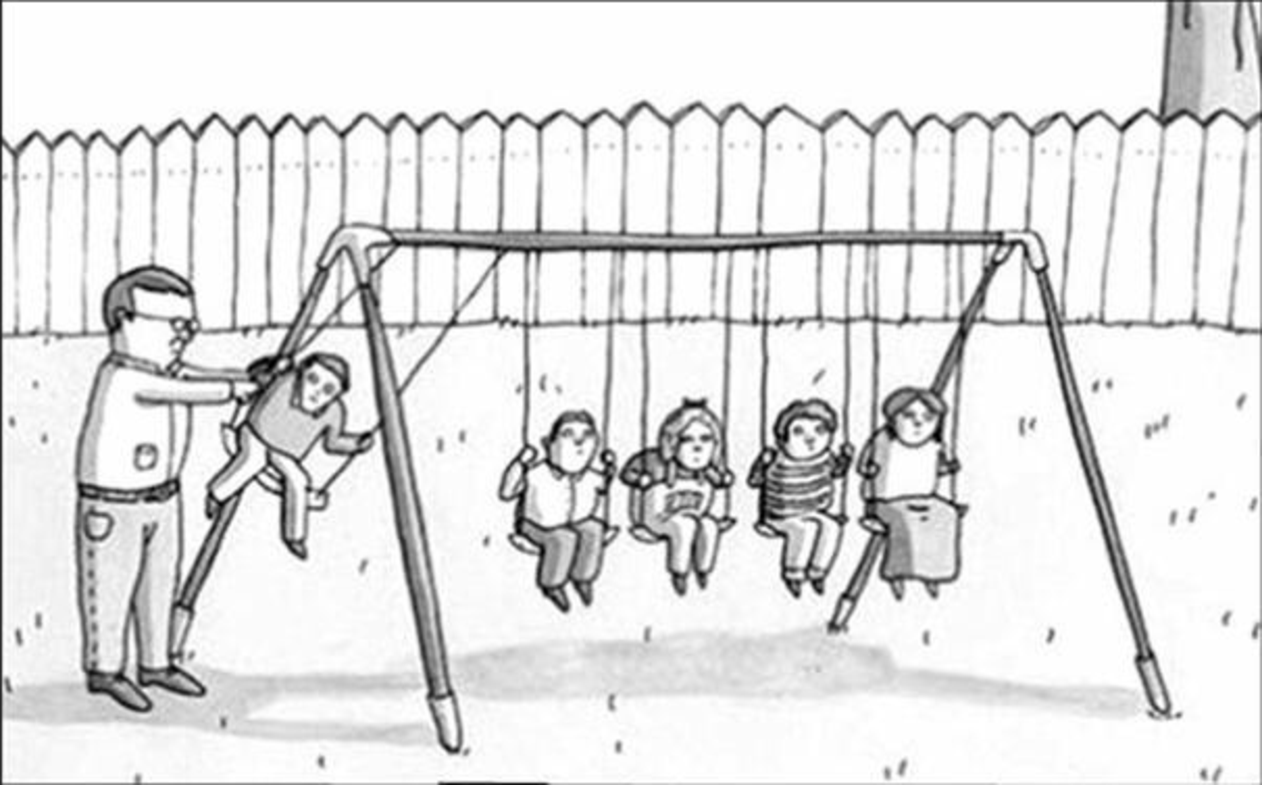
\includegraphics[height=1.5cm]{figures/experimentalist}}

                \end{columns}
            \end{center}
        }

    }

}

\slide[c]{

    \frametitle{Measurements $ P\left(\mathcal{D} | \boldsymbol{O} \right) $}

    \begin{itemize}
        \item $B\rightarrow K\mu^+\mu^-$: $\mathcal{B} , \red{A_{FB}} , \red{F_H}$
        \begin{itemize}
            \item \red{LHCb 2014 {\tiny (\href{http://arXiv.org/abs/1403.8044}{arXiv:1403.8044} , \href{http://arXiv.org/abs/1403.8045}{arXiv:1403.8045})}}
            \item CDF~ 2012 {\tiny (\url{http://www-cdf.fnal.gov/physics/new/bottom/120628.blessed-b2smumu_96})}
        \end{itemize}

        \item $B_s\rightarrow\mu^+\mu^-$: $\mathcal{B}$

        \begin{itemize}
            \item \red{LHCb+CMS 2014 {\tiny({\href{http://arXiv.org/abs/1411.4413}{arXiv:1411.4413}})}}
        \end{itemize}

        \item $B\rightarrow K^\ast\mu^+\mu^-$: $\mathcal{B}$

        \begin{itemize}
            \item LHCb 2013 {\tiny({\href{http://arXiv.org/abs/1304.6325}{arXiv:1304.6325}})}
            \item CMS~ 2013 {\tiny({\href{http://arXiv.org/abs/1308.3409}{arXiv:1308.3409}})}
            \item CDF~ 2012 {\tiny (\url{http://www-cdf.fnal.gov/physics/new/bottom/120628.blessed-b2smumu_96})}
        \end{itemize}
    \end{itemize}

}

\slide[c]{

    \frametitle{Parameters $\boldsymbol{\theta}$}

    {\large\textbf{scan parameters}}

    \begin{itemize}
        \item \red{Wilson coefficients $\mathcal{C}_{10} ^{(\prime)} , \mathcal{C}_S ^{(\prime)} , \mathcal{C}_P ^{(\prime)} , \mathcal{C}_T , \text{and} ~ \mathcal{C}_{T5}$}
    \end{itemize}

    \uncover<2->{{\large\textbf{nuisance parameters}}

    \begin{itemize}
        \item CKM matrix (4 parameters)
        \item charm and bottom quark mass (2 parameters)
        \item form factors
              \begin{itemize}
                  \item $B\rightarrow K^{\thinspace\thinspace\thinspace}$ (5 parameters)
                  \item $B\rightarrow K^\ast$                             (6 parameters)
              \end{itemize}
        \item $B_s$ decay constant $f_{B_s}$
        \item subleading corrections (11 parameters)
    \end{itemize}}

    \vspace{5mm}

    \uncover<3->{{\large\textbf{theory calculation $\boldsymbol{O(\theta , M)}$:}}

    \vspace{2.5mm}
    \Large open-source implementation: EOS-package \newline \large \url{http://project.het.physik.tu-dortmund.de/eos/}}

}

\slide[c]{

    \frametitle{Joint fit of $\mathcal{C}_{10} ^{(\prime)} , \mathcal{C}_S ^{(\prime)} , \mathcal{C}_P ^{(\prime)} , \mathcal{C}_T , \text{and} ~ \mathcal{C}_{T5}$}

    \vspace{6mm}

    \begin{columns}[c]
        \column{0.65\textwidth}
            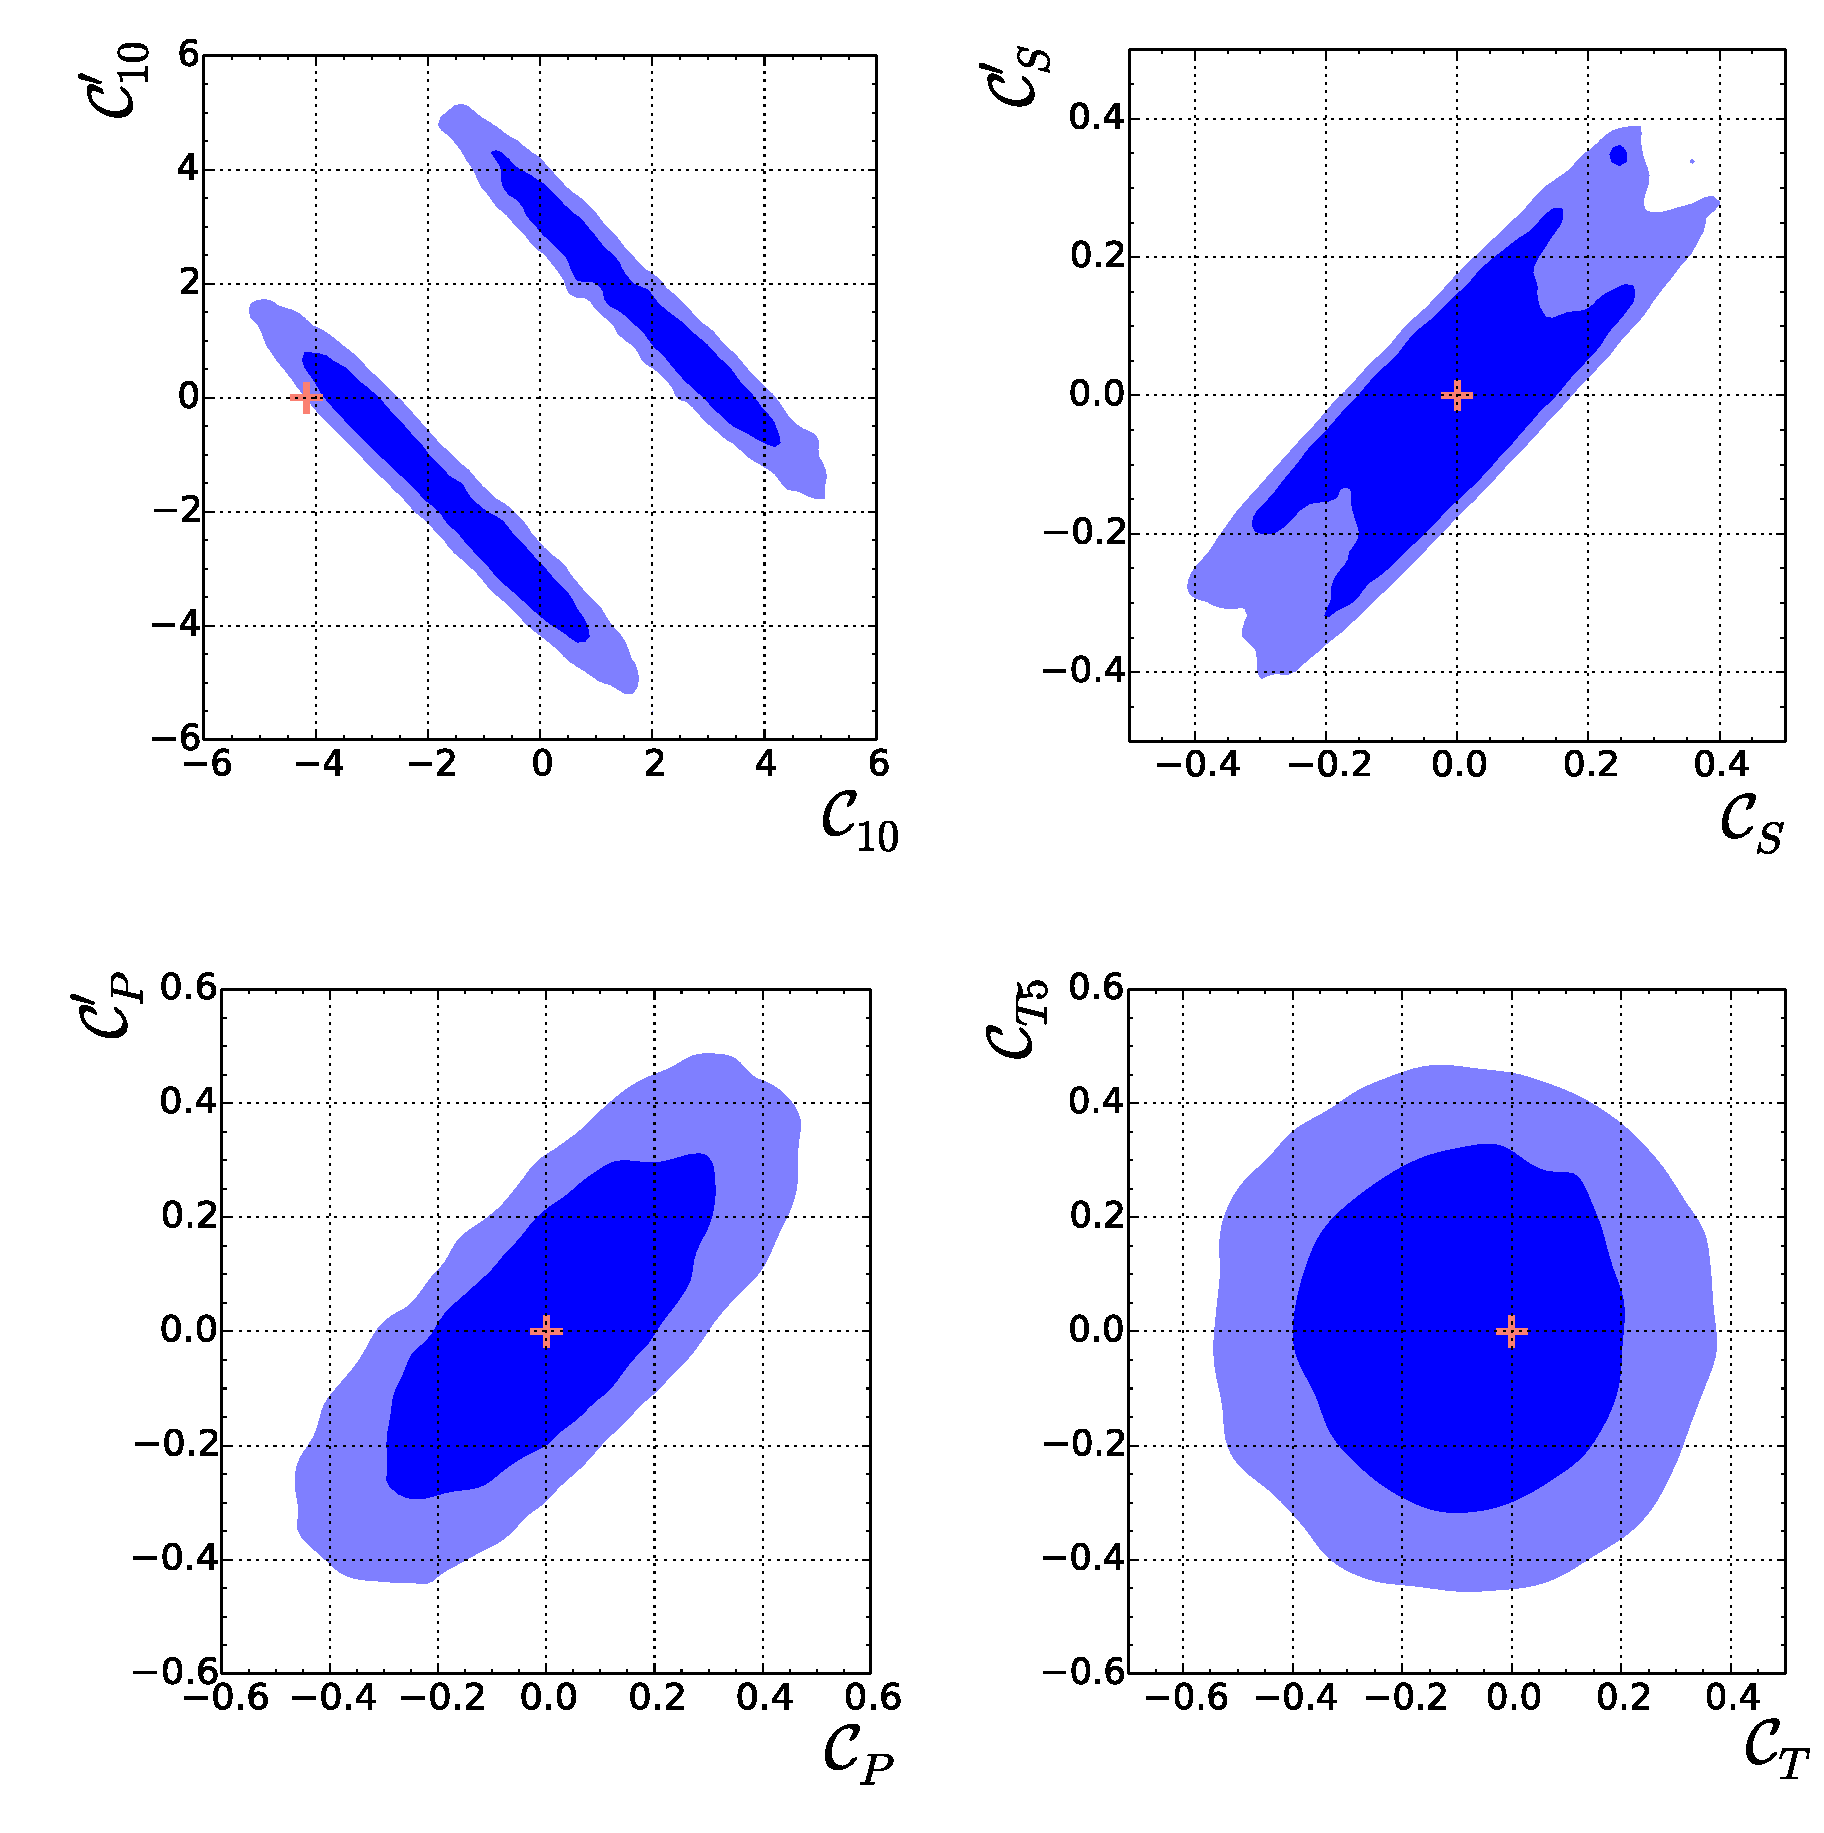
\includegraphics[width=\textwidth]{figures/Wilson_coeff_2d}

        \column{0.35\textwidth}
            \begin{itemize}
                \uncover<2->{\item first \emph{simultaneous} fit}
                \uncover<3->{\item interference $\mathcal{C}_{10} ^{(\prime)} \leftrightarrow \mathcal{C}_{S,P} ^{(\prime)}$
                        in $ \mathcal{B}(B_s\rightarrow \mu^+\mu^-) $
                            \begin{itemize}
                                \uncover<4->{\item[$\Rightarrow$] larger uncertainty than obtained for fixed $\mathcal{C}_{10} ^{(\prime)} = \mathcal{C}_{10} ^{(\prime) \mathrm{SM}}$ \newline {\tiny \href{http://arXiv.org/abs/1205.5811}{arXiv:1205.5811}, \href{http://arXiv.org/abs/1206.0273}{arXiv:1206.0273}, \href{http://arXiv.org/abs/1407.7044}{arXiv:1407.7044}}}
                            \end{itemize}
                      }
            \end{itemize}
            \vspace{6.5mm}

    \end{columns}

}

\section{Summary}

\slide[c]{

    \frametitle{\insertsectionhead}

    \begin{columns}[t] % [t]: top alignment; [c]: center alignment

        \column{0.5\textwidth}
            \uncover<2->{
                \begin{center}
                    {\begin{center}\large\textbf{algorithm to sample and integrate in $\boldsymbol{dim=\mathcal{O}(40)}$}\end{center}}
                    \vspace{9mm}
                    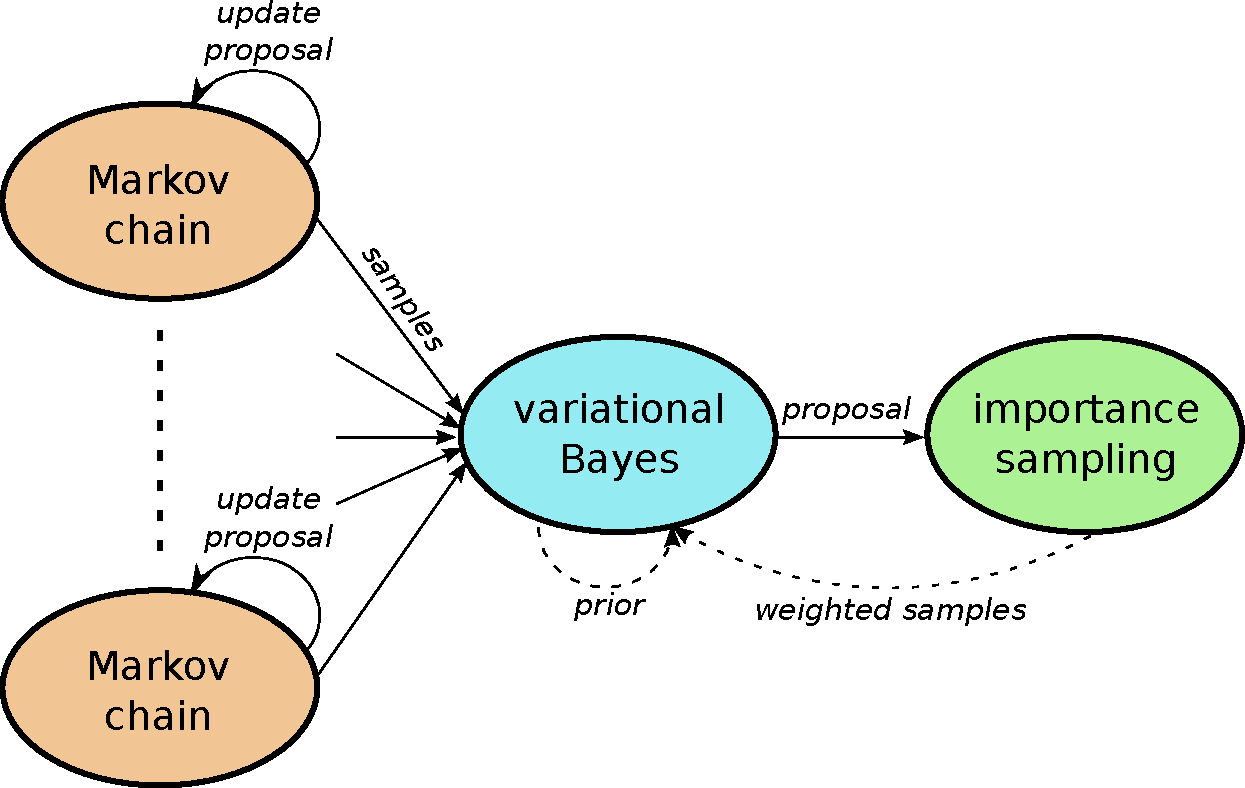
\includegraphics[width=0.9\textwidth]{figures/algorithm}
                \end{center}
            }


        \column{0.5\textwidth}
            \uncover<3->{
                {\begin{center}\large\textbf{model-independent search for new physics}\end{center}}

                \begin{itemize}
                    \uncover<4->{\item \red{simultaneous} fit of $\mathcal{C}_{10} ^{(\prime)} , \mathcal{C}_S ^{(\prime)} , \mathcal{C}_P ^{(\prime)} , \mathcal{C}_T , \text{and} ~ \mathcal{C}_{T5}$
                                 \begin{itemize} \item[$\Rightarrow$] updated constraints \end{itemize}} \

                    \uncover<5->{\item no significant deviation from the SM}
                    \newline
                    \uncover<6->{\item need better theoretical control}
                \end{itemize}
            }


    \end{columns}

}

\slide[t,nopagenumbering,noframenumbering]{

    \frametitle{Nuisance parameters}

    \begin{center}
        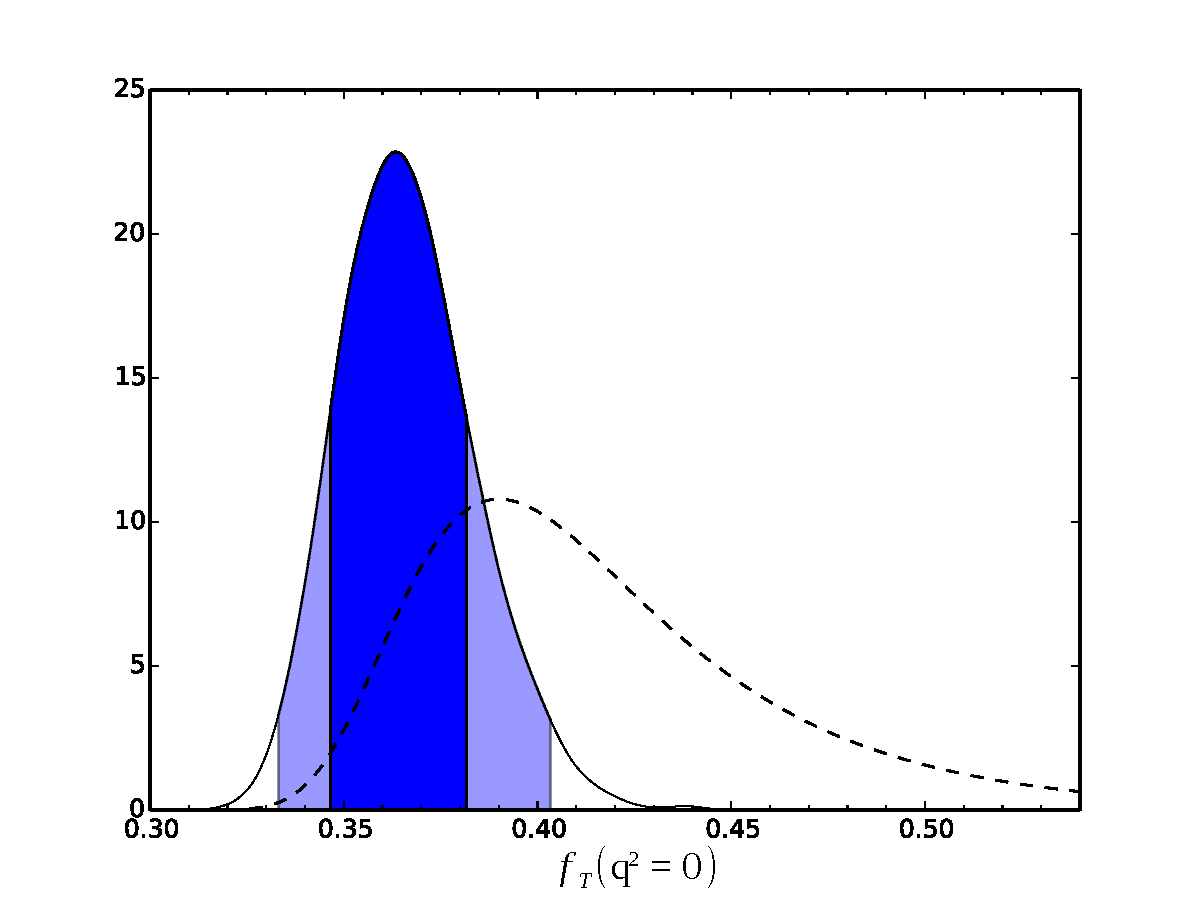
\includegraphics[width=0.9\textwidth]{figures/FF_ft0}
    \end{center}

}

\slide[nopagenumbering,noframenumbering]{

    \frametitle{Nuisance parameters}

    \begin{center}
        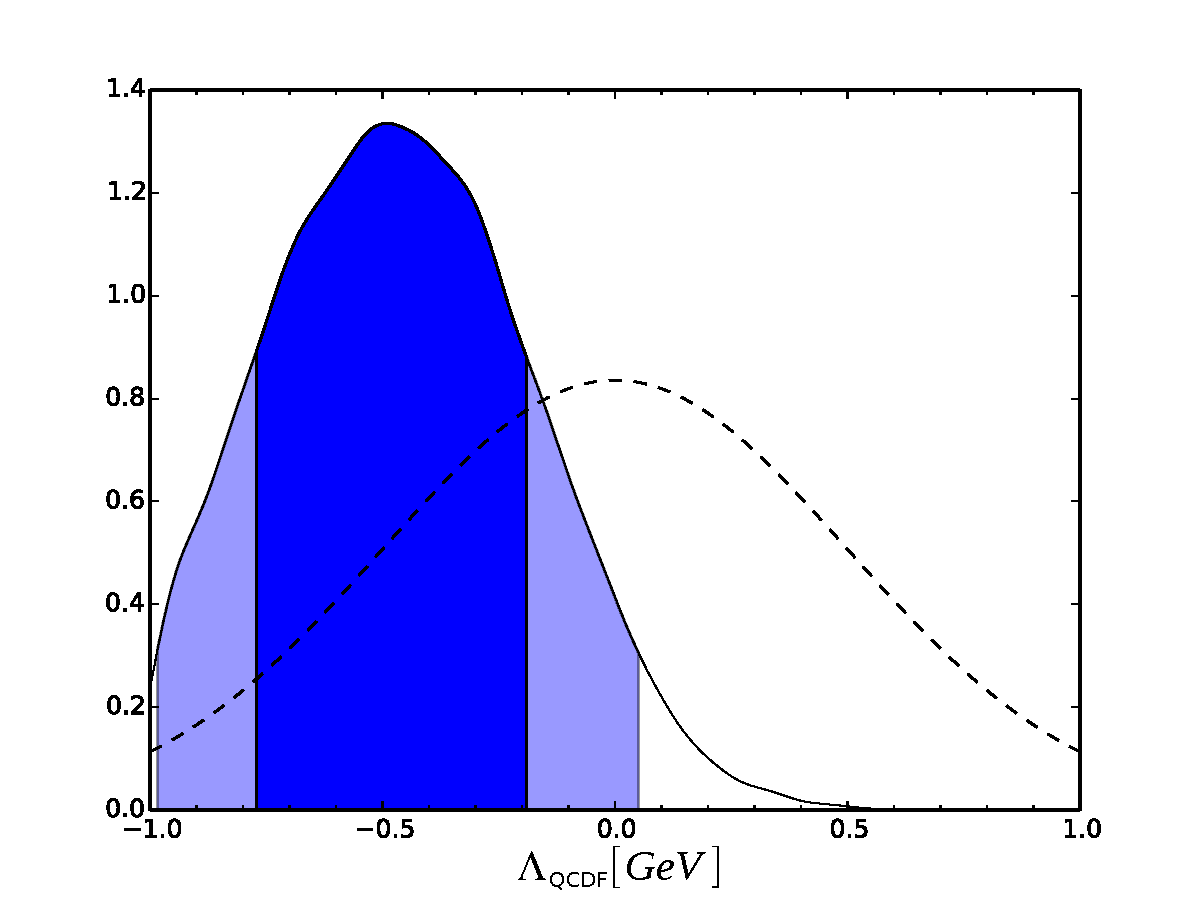
\includegraphics[width=0.9\textwidth]{figures/SL_large_recoil}
    \end{center}

}

\end{document}
